\documentclass[11pt]{article}
\usepackage[margin=1in]{geometry}
\usepackage{amsmath, amssymb}
\usepackage{graphicx}
\usepackage{booktabs}
\usepackage{hyperref}

\title{Evaluation of FNO-DeepONet for Black-Scholes Option Pricing}
\author{Experimental Framework Report}
\date{\today}

\begin{document}

\maketitle

\begin{abstract}
This document details the numerical experiments designed to rigorously evaluate the performance, physical consistency, and computational efficiency of the trained FNO-DeepONet model for solving the Black-Scholes partial differential equation. The evaluation encompasses global accuracy metrics, regime-specific error stratification, physical consistency of the Greeks, robustness to volatility regimes, and inference speed.
\end{abstract}

\section{Experiment 1: Global Error and Distribution Analysis}
The primary objective of this experiment is to establish the baseline accuracy of the model across the entire test dataset. Standard machine learning metrics are computed between the network's predicted normalized option price ($v_{hat}$) and the true normalized price ($v_{true}$). 

The metrics evaluated include:
\begin{itemize}
    \item \textbf{Mean Squared Error (MSE)} and \textbf{Root Mean Squared Error (RMSE)} to capture the variance of the residuals and penalize large deviations.
    \item \textbf{Mean Absolute Error (MAE)} for a robust average dollar-value error.
    \item \textbf{Mean Absolute Percentage Error (MAPE)} to assess relative error, which is particularly critical for out-of-the-money (OTM) options.
    \item \textbf{$\mathbf{R^2}$ Score} to quantify the proportion of the variance in the dependent variable that is predictable from the independent variables.
\end{itemize}

Additionally, the distribution of the residuals ($v_{hat} - v_{true}$) is analyzed. An unbiased, well-calibrated model is expected to exhibit a tight, zero-centered Gaussian distribution of residuals.

\begin{figure}[htpb]
    \centering
    % 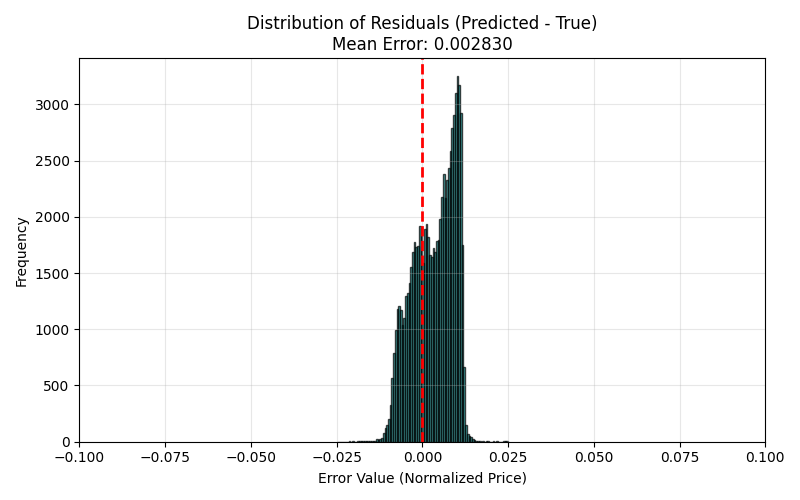
\includegraphics[width=0.6\textwidth]{exp1_residual_histogram.png}
    \vspace{2cm} % Placeholder space
    \caption{Placeholder for Residual Distribution Histogram.}
    \label{fig:exp1}
\end{figure}

\section{Experiment 2: Error Stratification Heatmap (Moneyness vs. Maturity)}
Financial models rarely fail uniformly; they tend to exhibit varying performance across different market regimes. This experiment stratifies the pricing error (MAE) across a two-dimensional grid defined by \textit{Moneyness} ($M = S/K$) and \textit{Time to Maturity} ($\tau$).

The test dataset is binned into the following categories:
\begin{itemize}
    \item \textbf{Moneyness ($M$):} Deep OTM ($M < 0.95$), OTM ($0.95 \le M < 0.98$), ATM ($0.98 \le M < 1.02$), ITM ($1.02 \le M < 1.05$), and Deep ITM ($M \ge 1.05$).
    \item \textbf{Maturity ($\tau$):} Short-term ($\tau < 0.1$ years), Medium-term ($0.1 \le \tau < 0.5$ years), and Long-term ($\tau \ge 0.5$ years).
\end{itemize}
The resulting heatmap provides immediate visual feedback on the regimes where the model excels and where it struggles (e.g., short-term OTM options, which represent a known challenge due to discontinuous payoff boundaries).

\section{Experiment 3: Evaluating the Greeks (Delta and Gamma)}
A critical advantage of Physics-Informed Neural Networks (PINNs) is their infinite differentiability. Option traders rely heavily on the derivatives of the price function with respect to the underlying asset (the ``Greeks'') for hedging purposes. 

Since the network predicts the normalized price $v = C/K$ using moneyness $M = S/K$, the derivatives obtained via PyTorch Automatic Differentiation directly correspond to the financial Greeks:
\begin{align}
    \Delta_{PINN} &= \frac{\partial v}{\partial M} = \frac{\partial (C/K)}{\partial (S/K)} = \frac{\partial C}{\partial S} \\
    \Gamma_{PINN} &= \frac{\partial^2 v}{\partial M^2} = \frac{\partial \Delta}{\partial (S/K)} = K \cdot \frac{\partial^2 C}{\partial S^2} = K \cdot \Gamma
\end{align}
This experiment computes the network's internal gradients $\frac{\partial v}{\partial M}$ and $\frac{\partial^2 v}{\partial M^2}$ using \texttt{torch.autograd.grad} and compares them against the analytical Black-Scholes Delta and normalized Gamma. Strong alignment validates that the model has learned the underlying PDE physics, not just the surface data points.

\section{Experiment 4: The FNO Branch Impact (Volatility Regimes)}
The FNO-DeepONet model is uniquely designed to process a continuous historical path of branch data ($u$, representing 11 days $\times$ 34 deltas). This experiment assesses how well the FNO branch adapts to different market volatility regimes.

The historical realized variance of the input path $u$ is computed for each sample in the test set. The dataset is then divided into quartiles, ranging from \textit{Low Volatility} to \textit{Extreme Volatility} environments. Comparing the pricing errors across these quartiles demonstrates the FNO branch's capacity to digest complex, real-time market turbulence and adjust the latent volatility parameter ($\sigma_{hat}$) accordingly.

\section{Experiment 5: Computational Efficiency Benchmark}
While neural networks require significant upfront training time, their inference speed is typically orders of magnitude faster than traditional numerical PDE solvers (like finite difference methods) or Monte Carlo simulations. 

This experiment benchmarks the model's computational efficiency during inference. The entire test dataset is passed through the network in batched forward passes, and the total execution time is recorded. The resulting throughput, measured in \textbf{options priced per second}, serves to justify the deployment of FNO-DeepONet in high-frequency trading or large-scale risk management scenarios where speed is paramount.

\end{document}
